% latex uft-8
\documentclass[uplatex,a4paper,11pt,oneside,openany]{jsbook}
% 
\usepackage[dvipdfmx]{graphicx}
\usepackage[dvipdfmx]{color}
\usepackage{amsmath,amssymb}
\usepackage{enumerate}
\usepackage{bm}
%\usepackage{graphicx}
\usepackage{ascmac}
\usepackage{setspace}
\usepackage{here}
\usepackage{listings,jlisting} %日本語のコメントアウトをする場合jlistingが必要
\usepackage{color}
%\lstset{
%  basicstyle={\ttfamily},
%  identifierstyle={\small},
%  commentstyle={\smallitshape},
%  keywordstyle={\small\bfseries},
%  ndkeywordstyle={\small},
%  stringstyle={\small\ttfamily},
%  frame={tb},
%  breaklines=true,
%  columns=[l]{fullflexible},
%  numbers=left,
%  xrightmargin=0zw,
%  xleftmargin=3zw,
%  numberstyle={\scriptsize},
%  stepnumber=1,
%  numbersep=1zw,
%  lineskip=-0.5ex
%}
%ここまでソースコードの表示に関する設定
%ここからソースコードの表示に関する設定
\lstset{
	%プログラム言語(複数の言語に対応,C,C++も可)
 	language = Python,
 	%背景色と透過度
 	backgroundcolor={\color[gray]{.95}},
 	%枠外に行った時の自動改行
 	breaklines = true,
 	%自動改行後のインデント量(デフォルトでは20[pt])
 	breakindent = 10pt,
 	%標準の書体
 	%basicstyle = \ttfamily\scriptsize,
  basicstyle=\fontsize{8}{10}\selectfont\ttfamily,
 	%コメントの書体
 	commentstyle = {\itshape \color[cmyk]{1,0.4,1,0}},
 	%関数名等の色の設定
 	classoffset = 0,
 	%キーワード(int, ifなど)の書体
 	keywordstyle = {\bfseries \color[cmyk]{0,1,0,0}},
 	%表示する文字の書体
 	stringstyle = {\ttfamily \color[rgb]{0,0,1}},
 	%枠 "t"は上に線を記載, "T"は上に二重線を記載
	%他オプション:leftline,topline,bottomline,lines,single,shadowbox
 	frame = TBrl,
 	%frameまでの間隔(行番号とプログラムの間)
 	framesep = 5pt,
 	%行番号の位置
 	numbers = left,
	%行番号の間隔
 	stepnumber = 1,
	%行番号の書体
 	numberstyle = \tiny,
	%タブの大きさ
 	tabsize = 4,
 	%キャプションの場所("tb"ならば上下両方に記載)
 	captionpos = t
}
%ここまでソースコードの表示に関する設定
\makeatletter
\def\ps@plainfoot{%
  \let\@mkboth\@gobbletwo
  \let\@oddhead\@empty
  \def\@oddfoot{\normalfont\hfil-- \thepage\ --\hfil}%
  \let\@evenhead\@empty
  \let\@evenfoot\@oddfoot}
  \let\ps@plain\ps@plainfoot
\renewcommand{\chapter}{%
  \if@openright\cleardoublepage\else\clearpage\fi
  \global\@topnum\z@
  \secdef\@chapter\@schapter}
\makeatother
%
\newcommand{\maru}[1]{{\ooalign{%
\hfil\hbox{$\bigcirc$}\hfil\crcr%
\hfil\hbox{#1}\hfil}}}
%
\setlength{\textwidth}{\fullwidth}
\setlength{\textheight}{40\baselineskip}
\addtolength{\textheight}{\topskip}
\setlength{\voffset}{-0.55in}
%
\begin{document}
% START DOCUMENT
%
% COVER
\begin{center}
  \huge \par
  \vspace{65mm}
  \huge \par
  \vspace{15mm}
  \LARGE Fractal Diagram \par
  \vspace{100mm}
  \Large \today \par
  \vspace{15mm}
  \Large S.Matoike \par
  \vspace{10mm}
  \Large \par
  \vspace{10mm}
\end{center}
\thispagestyle{empty}
\clearpage
\addtocounter{page}{-1}
\newpage
\setcounter{tocdepth}{3}
%
\tableofcontents
%
\chapter{はじめに}

フラクタル図形は、図形の一部を拡大すると、再び同じ形状の図形が現れる
という自己相似性と呼ばれる性質を持っている

%
\chapter{マンデルブロ集合}

漸化式

\begin{equation*}
 \left \{
\begin{array}{l}
z_{n+1}=z_n^2+c \qquad (c \in \mathbb{Z}) \\\\
x_0=0
\end{array}
\right.
\end{equation*}

において、$n \rightarrow \infty$で$z_n$が発散しないような複数数$c$の集合がマンデルブロ集合。

1980年、フラクタルの名付け親であった、ベノワ・マンデルブロによって発見された。\\

まず、$z=0$から計算を始めるので、
$z^2$に$c$を加えた結果は$c$である

これを元の$z$に代入すると、$ c^2+c$という結果が得られる

これを再び元の$z$に代入し、$(c^2+c)^2+c$を計算する

このように、1つ前の計算で得られた結果をもう一度$z$に代入して、順次計算を売り返していく

定数$c$が特別の値だと、計算を何度繰り返しても、$z^2+c$の大きさは、ある値を超えることはない

このような複素数$c$からなる集合をマンデルブロ集合という

複素平面上の$c$の位置毎に、繰返し回数$n$をプロットしていけばマンデルブロ集合を作図できる\\

数値計算なので、厳密な収束や発散の判定はできない

つまり、コンピュータは$\infty$回まで反復を続けられないので、反復回数の上限$maxItr$を定めておく

そこまで繰り返しても発散の判定に至らなかった時は、$maxItr$(或いは$0$)をその時の反復回数とする

発散の判定においても、適当に大きな数字$M$を定めておき、
$|z_n|$が$M$を超えたら発散と判定していく

これをプログラムした部分は、次の通り

\begin{lstlisting}[caption=複素数で計算,label=p1]
def Calculate(self, c): # c: Complex number
    # z0 = 0.0 + 1j*0.0
    z = c # z = z0**2 + c
    for n in range(self.maxItr):
        az = abs(z)
        if az > self.M:
            return n
        z = z*z + c
    return self.maxItr
\end{lstlisting}

上記反復計算は複素平面上の値$c$毎に呼び出され、
その$c$の時の反復回数$n$を
発散の速さを表す値として配列に格納していき、
計算終了後に、配列に納められた$n$に応じた色を$c$の位置に描画する

複素平面上のグリッドに対応する2次元配列に格納された計算結果$n$に
小さな値が入っているということは、それだけ速く発散したことに相当し、
逆に大きな値、特に上限値$maxItr$と等しい値(或いは$0$)が入っている場合は、
実際には発散しなかったとみなせる

発散しなかったときの複素平面上の値$c$は、
マンデルブロ集合に属する要素であるということ

Pythonは複素数型の変数を持っているので、
上記のようなプログラムの記述が可能だが、そうでない場合は
次の様にして、実数の領域での計算を行うことができる

\begin{lstlisting}[caption=実数で計算,label=p2]
def Calc(self, re, im): # re, im: Real number
    x = 0.0
    y = 0.0
    for n in range(self.maxItr):
        zx2 = x**2
        zy2 = y**2
        if zx2 + zy2 > self.M:
            return n
        x_ = zx2 - zy2 + re
        y_ = 2*x*y + im
        x, y = x_, y_
    return self.maxItr
\end{lstlisting}

結果を格納した2次元配列を、ヒートマップとしてmatplotlibで描画する

ここではnumpy.meshgridを使ってヒートマップを描いていく

\lstinputlisting[caption=マンデルブロ集合,label=p3]{../src/Mandel.py}
%
\begin{figure}[H]
  \centering
  \begin{tabular}{cc}
      \begin{minipage}{0.5\hsize}
      \centering
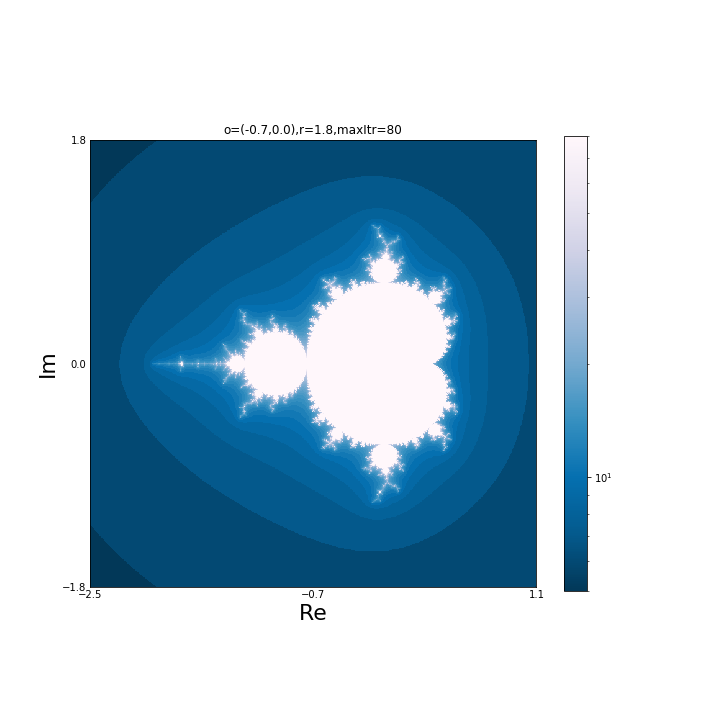
\includegraphics[bb=35 100 650 600,keepaspectratio,clip,scale=0.35]{../src/figure/mandel001.png}
      \end{minipage}
      \begin{minipage}{0.5\hsize}
      \centering
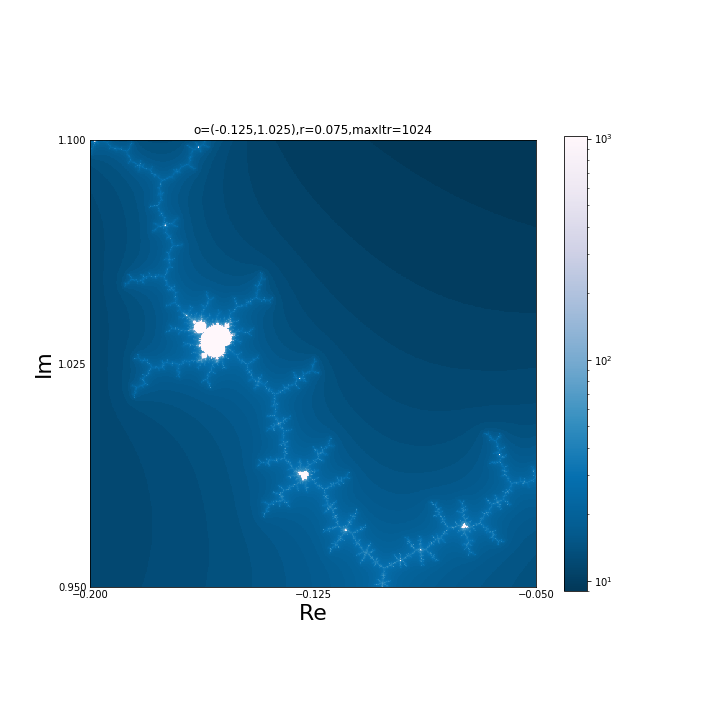
\includegraphics[bb=35 100 650 600,keepaspectratio,clip,scale=0.35]{../src/figure/mandel002.png}
      \end{minipage}
    \end{tabular}
\end{figure}%

\begin{figure}[H]
  \centering
    \begin{tabular}{cc}
      \begin{minipage}{0.5\hsize}
        \centering
  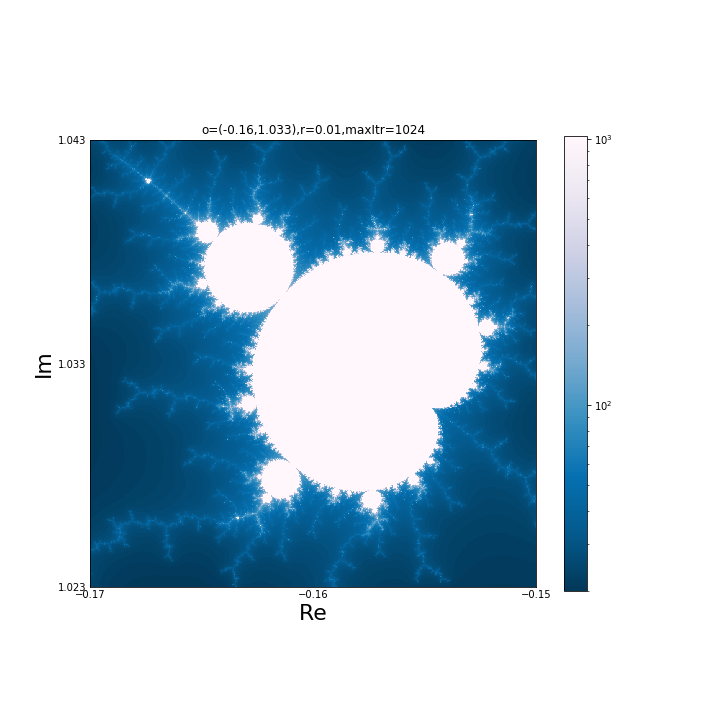
\includegraphics[bb=35 100 650 600,keepaspectratio,clip,scale=0.35]{../src/figure/mandel003.png}
      \end{minipage}
      \begin{minipage}{0.5\hsize}
        \centering
  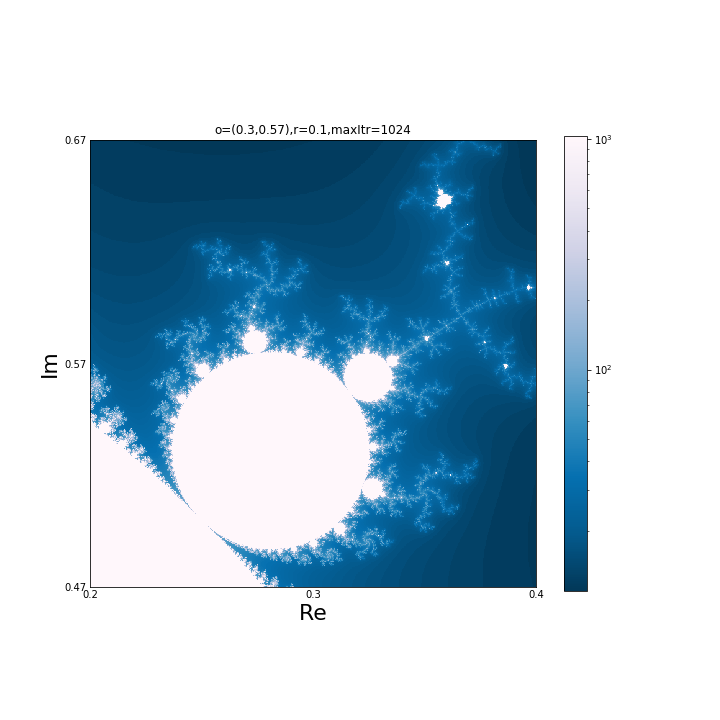
\includegraphics[bb=35 100 650 600,keepaspectratio,clip,scale=0.35]{../src/figure/mandel004.png}
      \end{minipage}
    \end{tabular}
\end{figure}%

\begin{figure}[H]
  \centering
    \begin{tabular}{cc}
      \begin{minipage}{0.5\hsize}
        \centering
  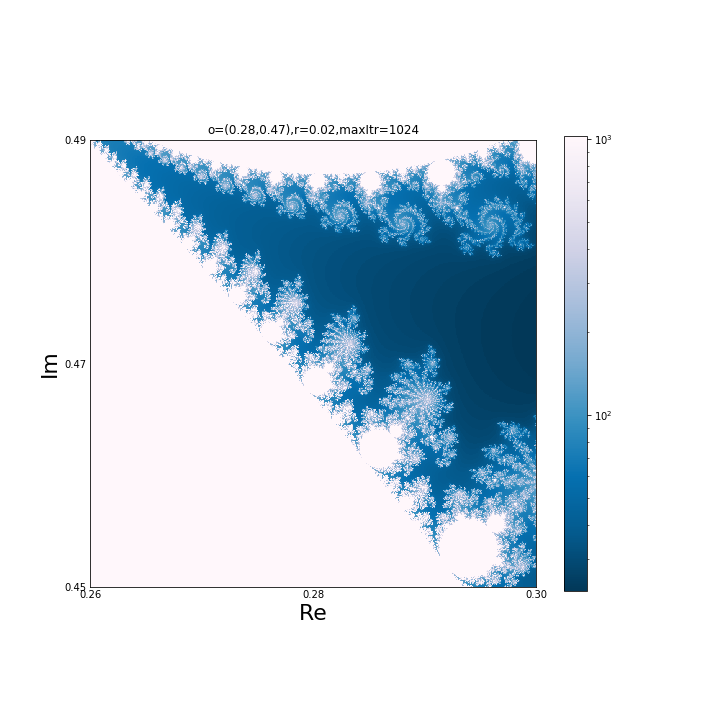
\includegraphics[bb=35 100 650 600,keepaspectratio,clip,scale=0.35]{../src/figure/mandel005.png}
      \end{minipage}
      \begin{minipage}{0.5\hsize}
        \centering
  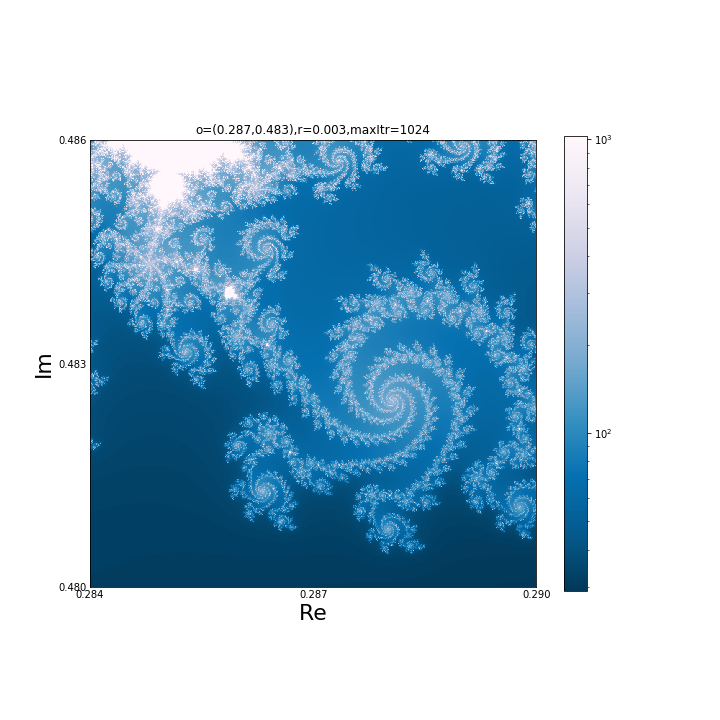
\includegraphics[bb=35 100 650 600,keepaspectratio,clip,scale=0.35]{../src/figure/mandel006.png}
      \end{minipage}
    \end{tabular}
\end{figure}%

\begin{figure}[H]
  \centering
    \begin{tabular}{cc}
      \begin{minipage}{0.5\hsize}
        \centering
  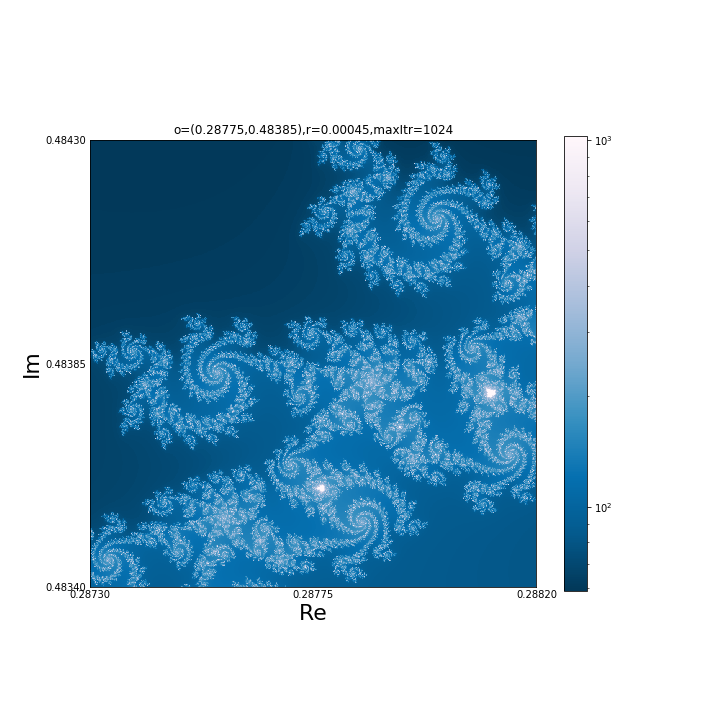
\includegraphics[bb=25 100 650 600,keepaspectratio,clip,scale=0.35]{../src/figure/mandel007.png}
      \end{minipage}
      \begin{minipage}{0.5\hsize}
        \centering
  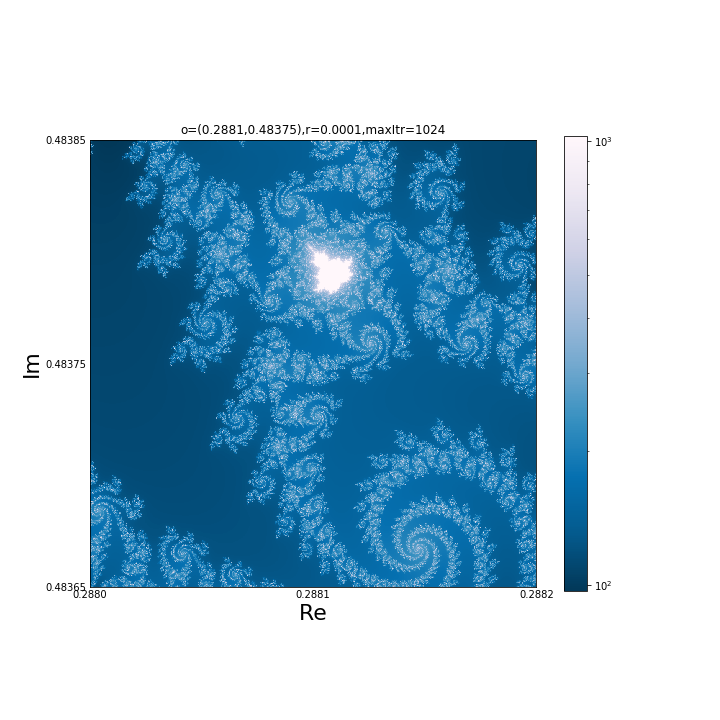
\includegraphics[bb=25 100 650 600,keepaspectratio,clip,scale=0.35]{../src/figure/mandel008.png}
      \end{minipage}
    \end{tabular}
\end{figure}%

\begin{figure}[H]
  \centering
    \begin{tabular}{cc}
      \begin{minipage}{0.5\hsize}
        \centering
  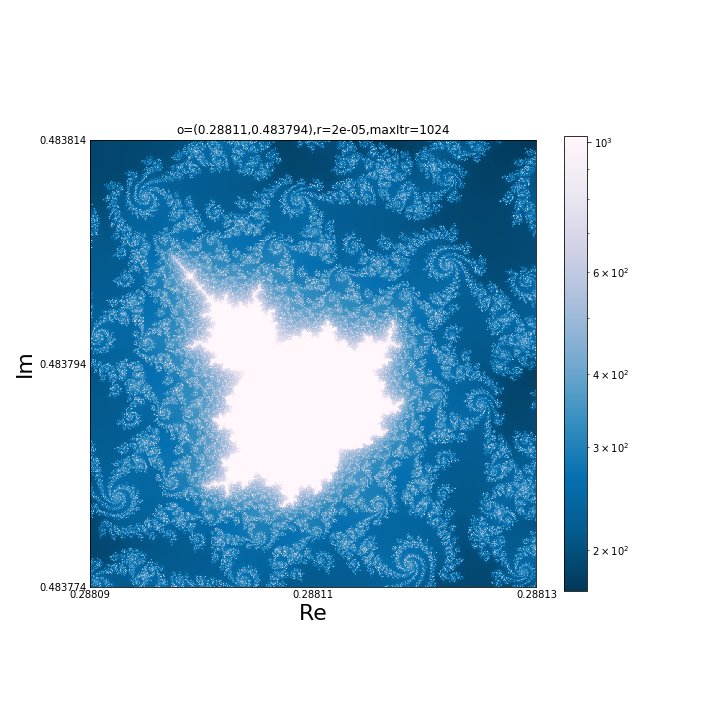
\includegraphics[bb=15 100 650 600,keepaspectratio,clip,scale=0.35]{../src/figure/mandel009.png}
      \end{minipage}
      \begin{minipage}{0.5\hsize}
        \centering
  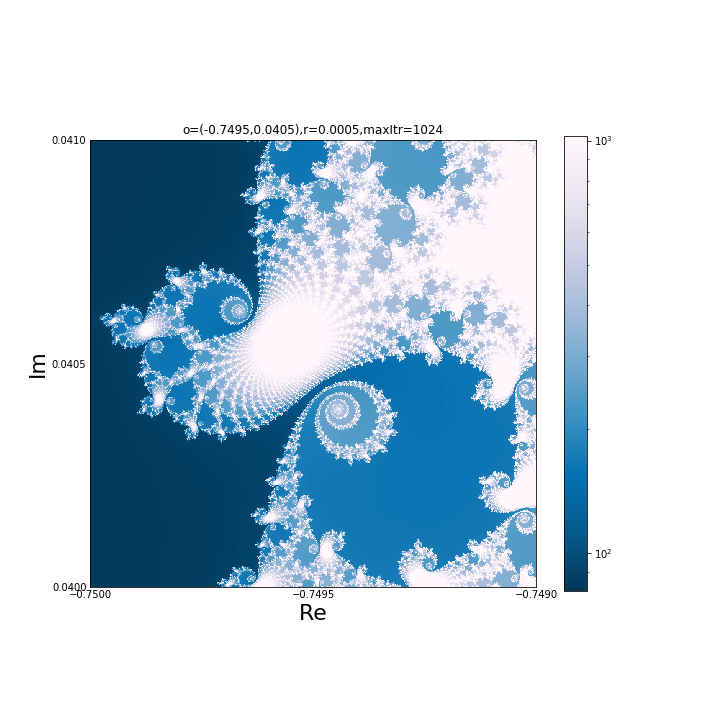
\includegraphics[bb=15 100 650 600,keepaspectratio,clip,scale=0.35]{../src/figure/mandel010.png}
      \end{minipage}
    \end{tabular}
\end{figure}%

\newpage

【別解】

\lstinputlisting[caption=マンデルブロー集合,label=p9]{../src/mandelbrotset.py}

\newpage

max\_iterが大きいと、この程度の画素(n=1000)では境界周辺が塗りつぶされて描かれない

\begin{figure}[H]
  \centering
  \begin{tabular}{cc}
      \begin{minipage}{0.9\hsize}
      \centering
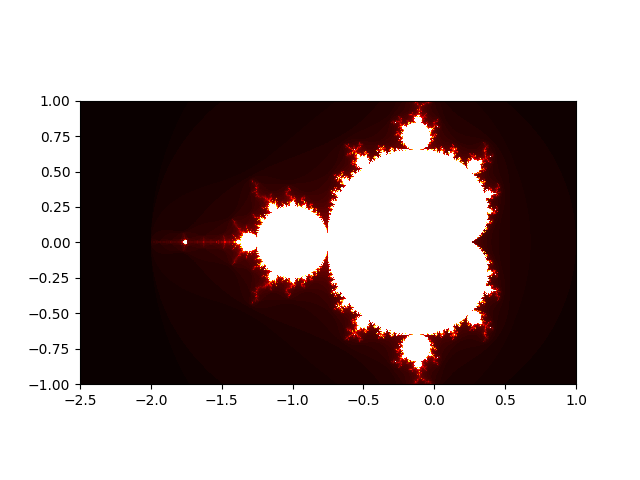
\includegraphics[keepaspectratio,clip,scale=0.8]{../src/figure/mandelbrotset0.png}
\caption{n=1000, max\_iter=100, 02:05 elapsed}
      \end{minipage}
      \begin{minipage}{0.1\hsize}
      \centering
%\includegraphics[keepaspectratio,clip,scale=0.5]{fern.png}
      \end{minipage}
    \end{tabular}
\end{figure}%

max\_iterを大きくしないと、白い部分の詳細が描かれない

\begin{figure}[H]
  \centering
  \begin{tabular}{cc}
      \begin{minipage}{0.5\hsize}
      \centering
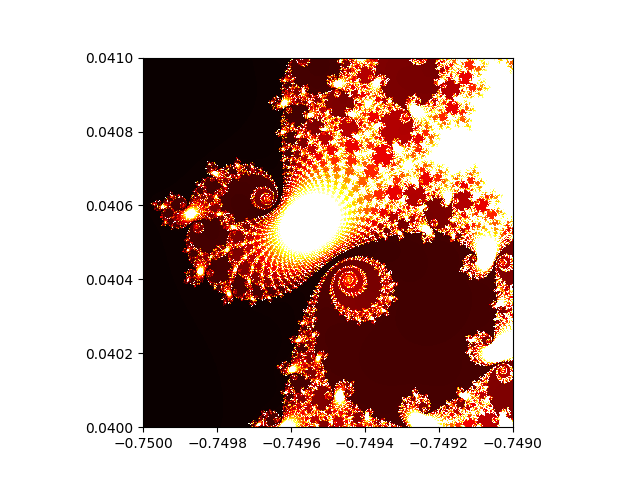
\includegraphics[keepaspectratio,clip,scale=0.5]{../src/figure/mandelbrotset.png}
\caption{n=1000, max\_iter=1000,19:18 elapsed}
      \end{minipage}
      \begin{minipage}{0.5\hsize}
      \centering
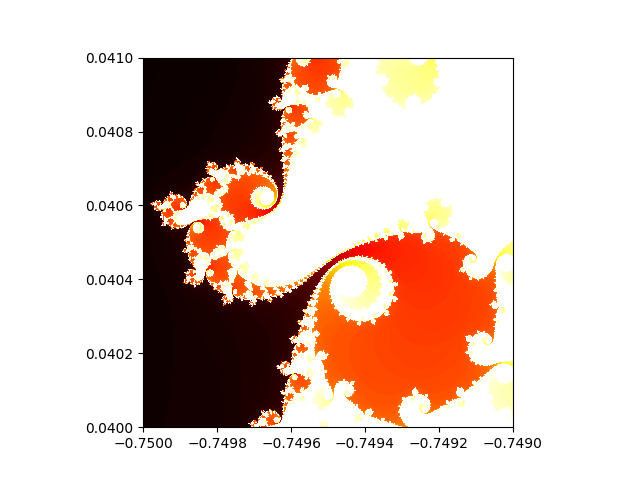
\includegraphics[keepaspectratio,clip,scale=0.5]{../src/figure/mandelbrotset1.png}
\caption{n=1000, max\_iter=250, 15:36 elapsed}
      \end{minipage}
    \end{tabular}
\end{figure}%

%\includegraphics[keepaspectratio,clip,scale=0.5]{mandelbrotset2.png}
%\caption{n=1000, max\_iter=500, 17:43 elapsed}

\chapter{ジュリア集合}

漸化式はマンデルブロ集合の場合と同じままで、
$c \quad (\in \mathbb{Z})$は予め定数として固定しておき、
$z_0$を変数として、複素平面上の点を順に与えて計算した時に、
漸化式が発散しないような$z_0$を要素とする集合は、
Julia(ジュリア)集合と呼ばれる

実際のプログラムは次の通り

\begin{lstlisting}[caption=複素数で計算,label=p4]
def Calculate(self, z0): # z0: Complex number
    z = z0
    for n in range(self.maxItr):
        az = abs(z)
        if az > self.M:
            return n
        z = z*z + self.c
    return self.maxItr
\end{lstlisting}

なお、実数の世界で計算するならば、

\begin{lstlisting}[caption=実数で計算,label=p5]
def Calc(self, re, im): # re, im: Real number
    z_r = re
    z_i = im
    for n in range(self.maxItr):
        zr2 = z_r**2
        zi2 = z_i**2
        if zr2 + zi2 > self.M:
            return n
        z_r_ = zr2 - zi2 + self.c_r
        z_i_ = 2*z_r*z_i + self.c_i
        z_r, z_i = z_r_, z_i_
    return self.maxItr
\end{lstlisting}

ここでも発散の速度をヒートマップにすることで、グラフを可視化することができる

複素定数の$c$(プログラム中の$c\_r$と$c\_i$)を変えると、色々なグラフが得られる

\lstinputlisting[caption=ジュリア集合,label=p6]{../src/Julia.py}

\begin{figure}[H]
  \centering
  \begin{tabular}{cc}
      \begin{minipage}{0.5\hsize}
      \centering
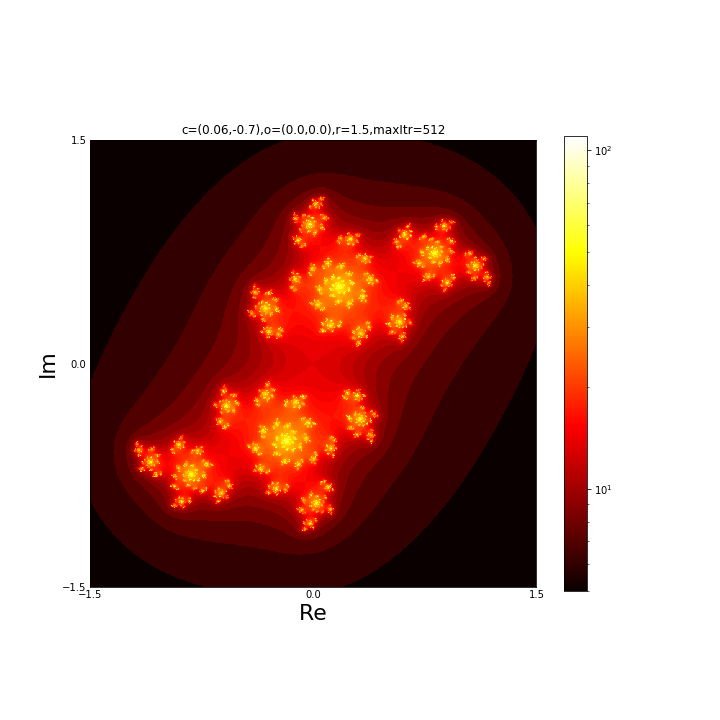
\includegraphics[bb=35 100 650 600,keepaspectratio,clip,scale=0.35]{../src/figure/julia001.png}
      \end{minipage}
      \begin{minipage}{0.5\hsize}
      \centering
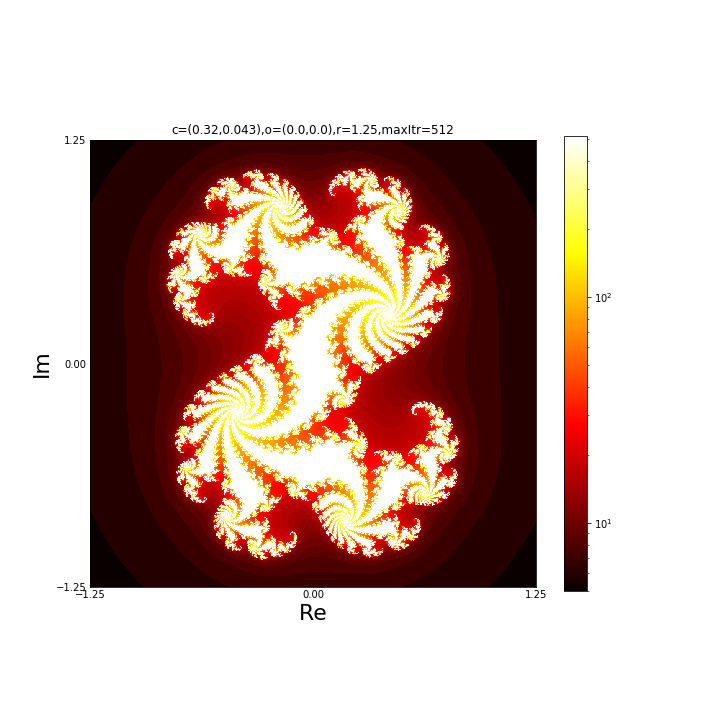
\includegraphics[bb=35 100 650 600,keepaspectratio,clip,scale=0.35]{../src/figure/julia002.png}
      \end{minipage}
    \end{tabular}
\end{figure}%

\begin{figure}[H]
  \centering
  \begin{tabular}{cc}
      \begin{minipage}{0.5\hsize}
      \centering
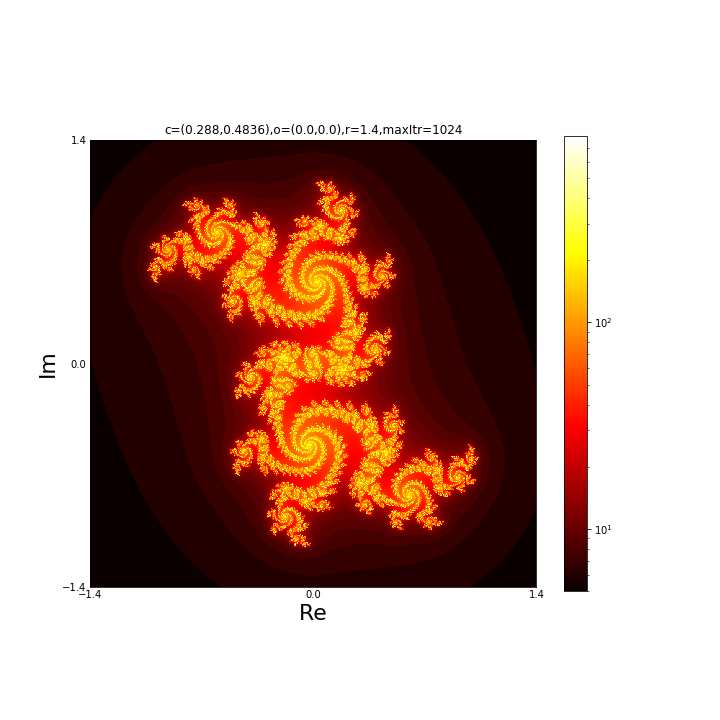
\includegraphics[bb=35 100 650 600,keepaspectratio,clip,scale=0.35]{../src/figure/julia004.png}
      \end{minipage}
      \begin{minipage}{0.5\hsize}
      \centering
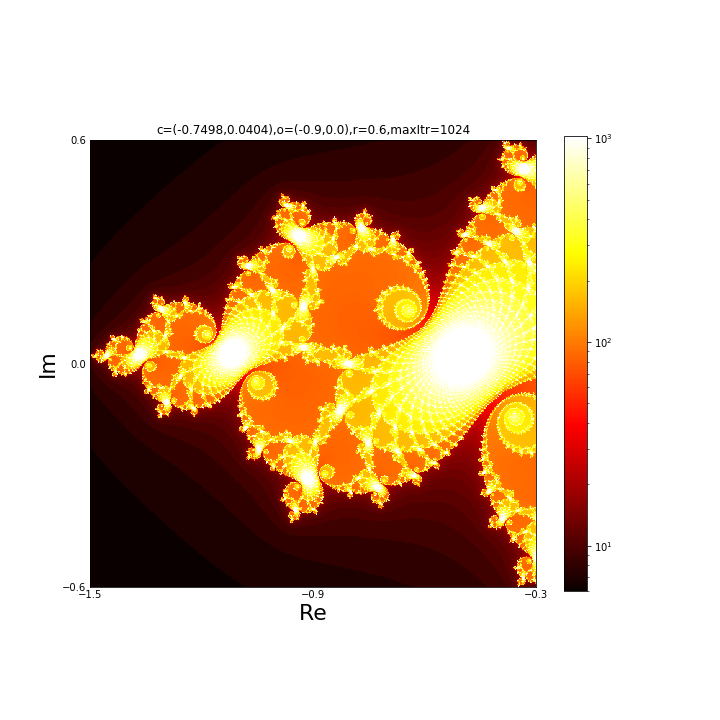
\includegraphics[bb=35 100 650 600,keepaspectratio,clip,scale=0.35]{../src/figure/julia003.png}
      \end{minipage}
    \end{tabular}
\end{figure}%

\begin{figure}[H]
  \centering
  \begin{tabular}{cc}
      \begin{minipage}{0.5\hsize}
      \centering
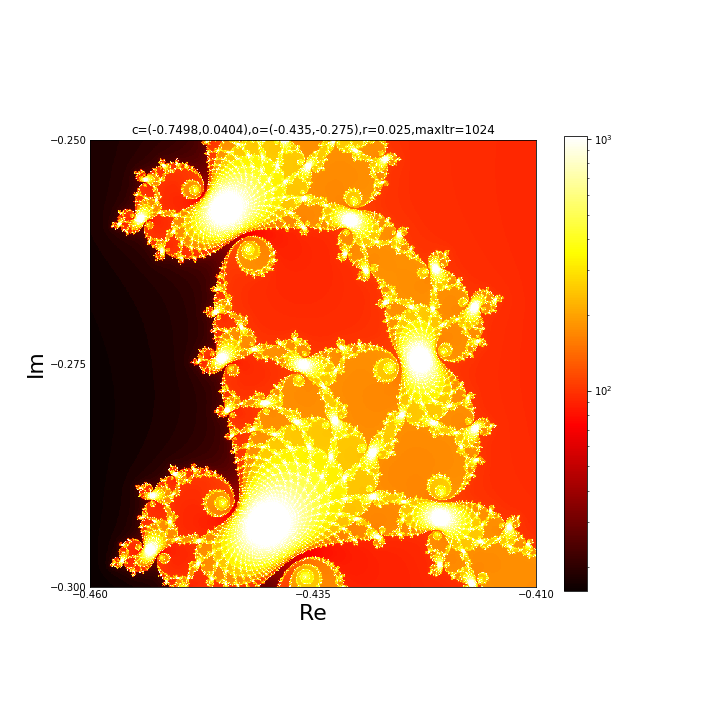
\includegraphics[bb=25 100 650 600,keepaspectratio,clip,scale=0.35]{../src/figure/julia006.png}
      \end{minipage}
      \begin{minipage}{0.5\hsize}
      \centering
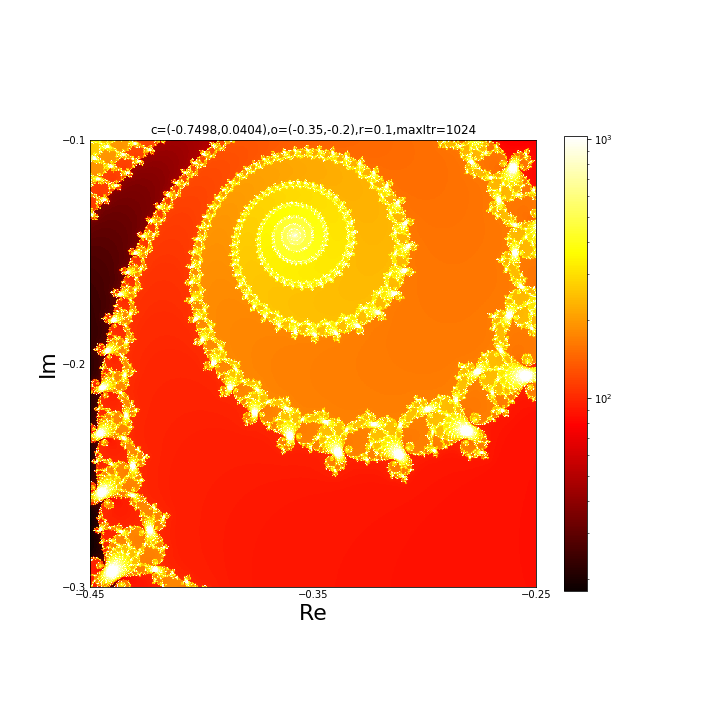
\includegraphics[bb=35 100 650 600,keepaspectratio,clip,scale=0.35]{../src/figure/julia005.png}
      \end{minipage}
    \end{tabular}
\end{figure}%

\chapter{再帰的処理による図形}

\section{コッホ曲線}

Helge von Koch が考案したフラクタル図形

\begin{figure}[H]
  \centering
  \begin{tabular}{cc}
      \begin{minipage}{0.5\hsize}
      \centering
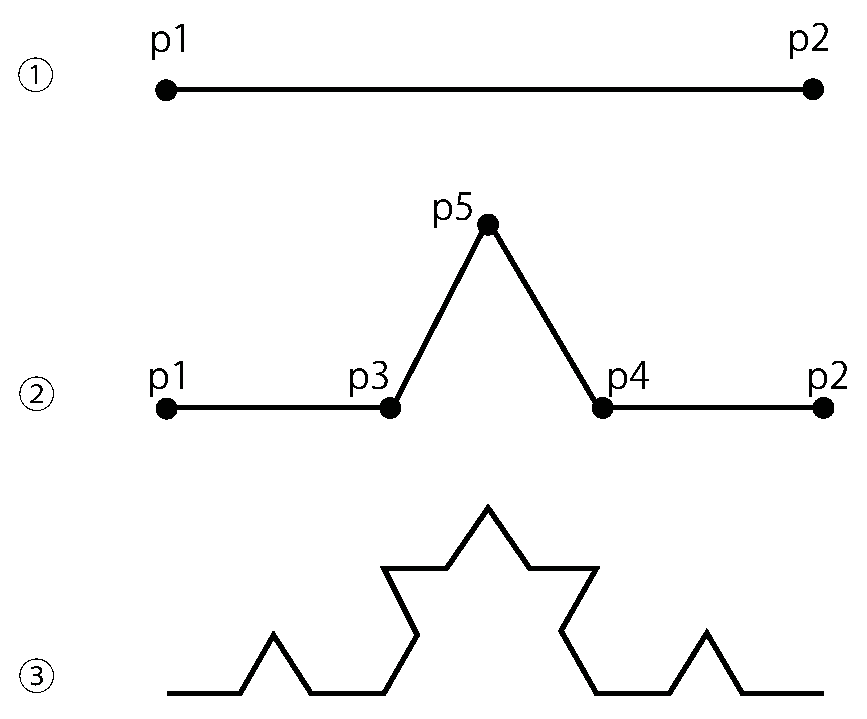
\includegraphics[keepaspectratio,clip,scale=0.45]{../src/figure/kochf1.eps}
      \end{minipage}
      \begin{minipage}{0.5\hsize}
      \centering
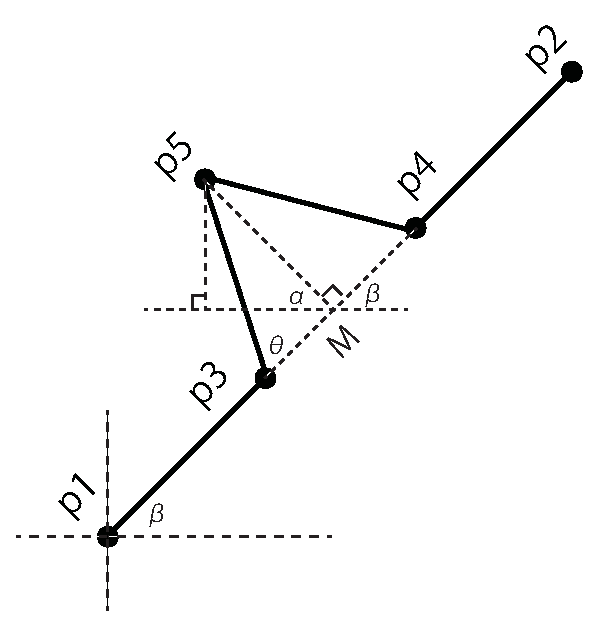
\includegraphics[keepaspectratio,clip,scale=0.55]{../src/figure/kochf4.eps}
      \end{minipage}
    \end{tabular}
\end{figure}%

①の線分$p_1(x_1,y_1)$、$p_2(x_2,y_2)$が与えられて、$p_3,p_4,p_5$の座標を求める問題を考える

例えば、点$p_3(x_3,y_3)$ならば次の通り

\begin{equation}
  x_3 = x_1 + \frac{x_2-x_1}{3} = \frac{1}{3}(2x_1+x_2), \qquad y_3 = y_1 + \frac{y_2-y_1}{3} = \frac{1}{3}(2y_1+y_2)
\end{equation}

$p_4(x_4,y_4)$も同様に

\begin{equation}
  x_4 = x_1 + \frac{2(x_2-x_1)}{3} = \frac{1}{3}(x_1+2x_2), \qquad y_4 = y_1 + \frac{2(y_2-y_1)}{3} = \frac{1}{3}(y_1+2y_2)
\end{equation}

点$p_5$の座標は、点$p_1$と点$p_2$の中間点$M(x_M,y_M)$を基準に計算を進める

\begin{equation*}
  x_M = x_1 + \frac{1}{2}(x_2-x_1)=\frac{1}{2}(x_1+x_2), \qquad y_M = y_1 + \frac{1}{2}(y_2-y_1)=\frac{1}{2}(y_1+y_2)
\end{equation*}

辺$p_1p_3$、辺$p_3p_4$、辺$p_4p_2$、そして辺$p_3p_5$、辺$p_5p_4$の長さ$l$は等しくて、

\begin{equation*}
    l=\sqrt{(x_4-x_3)^2+(y_4-y_3)^2}=\frac{1}{3}\sqrt{(x_2-x_1)^2+(y_2-y_1)^2}
\end{equation*}

また、正三角形なので$\theta=\pi/3$[rad]より、
その正三角形の高さは$h=l\sin\theta=l\sqrt{3}/2$で求まる

\begin{equation}
  x_5 = x_M-h\cos\alpha, \qquad y_5 = y_M+h\sin\alpha \qquad (但し \alpha=\frac{\pi}{2}-\beta)
\end{equation}

ここで、角度$\beta$ は、

\begin{equation*}
    \beta=\tan^{-1}\left({\frac{y_2-y_1}{x_2-x_1}}\right)
\end{equation*}

となるのだが、$x_2-x_1$が$0$になる場合(即ち$x_1=x_2$の場合、この時$y_5=y_M$、あるいは$\beta$が$\pi/2$や$3\pi/4$になる)、
$\tan$や$\arctan$は計算できないので、プログラム上では特別扱いが必要になる

即ち、$x_1=x_2$の時、

\begin{equation*}
  x_5=x_M-h, \qquad y_5=y_M, \qquad (但し、h=l\sin\frac{\pi}{3} = l\frac{\sqrt{3}}{2})
\end{equation*}

$p1$の$y$座標が$p2$の$y$座標より小さいとき、$p5$は左へ飛び出しているが、
$p1$の$y$座標が$p2$の$y$座標より大きいとき、$p5$は右へ飛び出しているので、
上の式の$x_5=x_M-h$で$h$の符号を反転させる必要がある

\lstinputlisting[caption=コッホの曲線,label=p8]{../src/koch.py}

\begin{figure}[H]
  \centering
  \begin{tabular}{cc}
      \begin{minipage}{0.9\hsize}
      \centering
\includegraphics[keepaspectratio,clip,scale=0.7]{../src/figure/figkoch1.png}
      \end{minipage}
      \begin{minipage}{0.1\hsize}
      \centering
%\includegraphics[keepaspectratio,clip,scale=0.5]{figkoch2.png}
      \end{minipage}
    \end{tabular}
\end{figure}%

%\newpage

\subsection{コッホの雪片曲線}

\lstinputlisting[caption=コッホの雪片曲線,label=p9]{../src/koch2.py}

\begin{figure}[H]
  \centering
  \begin{tabular}{cc}
      \begin{minipage}{0.1\hsize}
      \centering
%\includegraphics[keepaspectratio,clip,scale=0.5]{figkoch1.png}
      \end{minipage}
      \begin{minipage}{0.9\hsize}
      \centering
\includegraphics[keepaspectratio,clip,scale=0.7]{../src/figure/figkoch2.png}
      \end{minipage}
    \end{tabular}
\end{figure}%

\newpage

\section{シェルピンスキーの三角形}

Waclaw Sierpinski's gasket

\begin{figure}[H]
  \centering
  \begin{tabular}{cc}
      \begin{minipage}{0.5\hsize}
      \centering
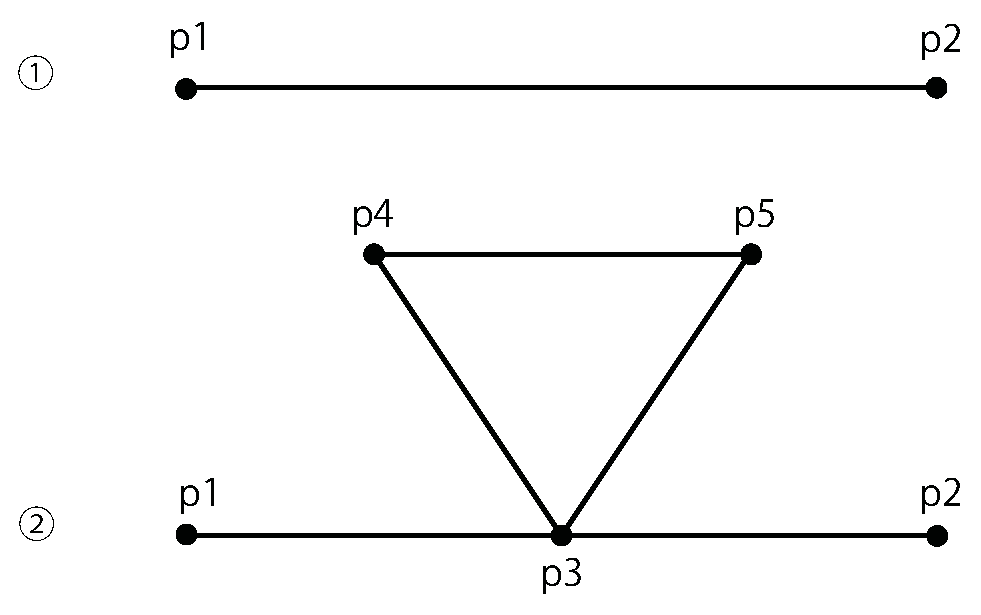
\includegraphics[keepaspectratio,clip,scale=0.45]{../src/figure/kochf2.eps}
      \end{minipage}
      \begin{minipage}{0.5\hsize}
      \centering
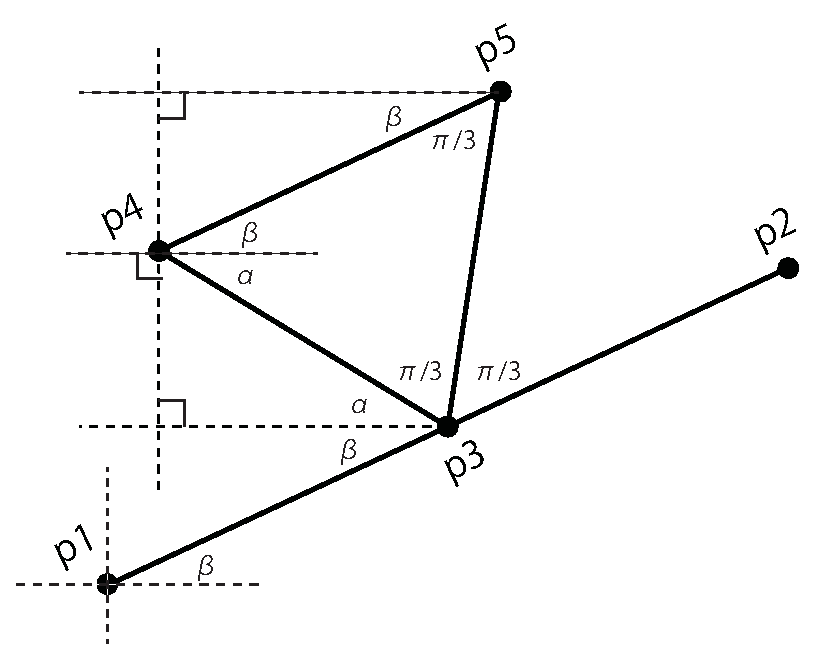
\includegraphics[keepaspectratio,clip,scale=0.45]{../src/figure/kochf5.eps}
      \end{minipage}
    \end{tabular}
\end{figure}%

①の線分が2つの点$p_1,p_2$によって与えられた時に、3つの点$p_3,p_4,p_5$の座標を求める問題を考える

点$p_3(x_3,y_3)$は、2つの点$p_1$と$p_2$の中点である

\begin{equation}
  x_3=x_1+\frac{x_2-x_1}{2}=\frac{1}{2}(x_1+x_2), \qquad y_3=y_1+\frac{y_2-y_1}{2}=\frac{1}{2}(y_1+y_2)
\end{equation}

辺$p_1p_3$、辺$p_3p_4$、辺$p_4p_5$、辺$p_5p_3$、及び辺$p_3p_2$の長さ$l$は等しくて

\begin{equation*}
  l=\frac{\sqrt{(x_2-x_1)^2+(y_2-y_1)^2}}{2}
\end{equation*}

従って、三角形$p_3$ $p_4$ $p_5$は正三角形である

点$p_4(x_4,y_4)$は、角度$\alpha$と辺の長さ$l$を使って、

\begin{equation}
  x_4=x_3-l\cos\alpha, \qquad y_4=y_3+l\sin\alpha \qquad 但し、\alpha=\frac{\pi}{3}-\beta
\end{equation}

ここで、$\beta$は次の様にして予め計算しておく必要があります

\begin{equation*}
  \beta=\tan^{-1}\left(\frac{y_2-y_1}{x_2-x_1}\right)
\end{equation*}

この$\beta$は$x_1=x_2$の時に$\arctan$や$\tan$は計算できないので、
プログラム上の特別扱いが必要です

即ち$x_1=x_2$の時というのは、$\beta$が$\pi/2$[rad]あるいは$3\pi/4$[rad]の場合ですが、

\begin{equation*}
  y_4=y_1+\frac{l}{2}, \quad y_5=y_3+\frac{l}{2}, \quad x_4=x_5=x_1-h, \quad (但し、h=l\sin\frac{\pi}{3}=l\frac{\sqrt{3}}{2})
\end{equation*}

ここまでに計算した$p_4(x_4,y_4)$を元にして$p_5(x_5,y_5)$を求めます

\begin{equation}
  x_5=x_4+l\cos\beta, \qquad y_5=y_4+l\sin\beta
\end{equation}

\newpage

【別解】

\lstinputlisting[caption=シェルピンスキーの三角形,label=p8]{../src/sierpinski.py}

%\section{ケーリーツリー}
%\lstinputlisting[caption=コッホ曲線,label=p7]{Koch2.py}

%\lstinputlisting[caption=コッホ曲線,label=p8]{Koch.py}

\begin{figure}[H]
  \centering
  \begin{tabular}{cc}
      \begin{minipage}{0.9\hsize}
      \centering
\includegraphics[keepaspectratio,clip,scale=0.6]{../src/figure/sierpinski.png}
      \end{minipage}
      \begin{minipage}{0.1\hsize}
      \centering
%\includegraphics[keepaspectratio,clip,scale=0.5]{fern.png}
      \end{minipage}
    \end{tabular}
\end{figure}%

\section{バーンスレイのシダ}

Michael Barnsley

\lstinputlisting[caption=バーンスレイのシダ,label=p7]{../src/fern.py}

\begin{figure}[H]
  \centering
  \begin{tabular}{cc}
      \begin{minipage}{0.1\hsize}
      \centering
%\includegraphics[keepaspectratio,clip,scale=0.5]{sierpinski.png}
      \end{minipage}
      \begin{minipage}{0.9\hsize}
      \centering
\includegraphics[keepaspectratio,clip,scale=0.6]{../src/figure/fern.png}
      \end{minipage}
    \end{tabular}
\end{figure}%


\chapter{おわりに}

参考にした記事より(おまけ)

https://nepia01.blogspot.com/2017/07/python.html

\lstinputlisting[caption=参考記事,label=p7]{../src/Mandelbrot.py}

cmap='hogehoge'で指定するhogehogeは、以下に一覧がある

https://matplotlib.org/examples/color/colormaps\_reference.html

\newpage

\begin{figure}[H]
  \centering
  \begin{tabular}{cc}
    \begin{minipage}{0.5\hsize}
      \centering
      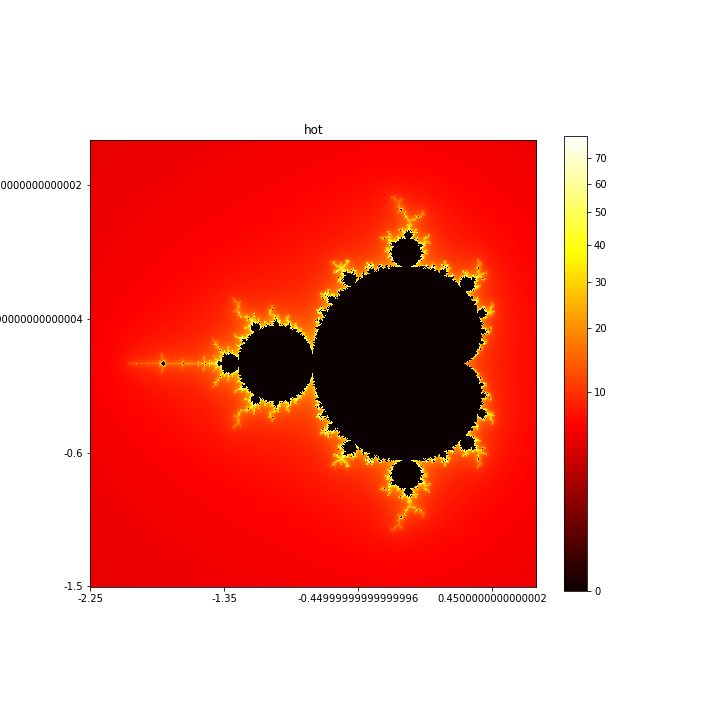
\includegraphics[clip,scale=0.3]{../src/figure/fig001.png}
    \end{minipage}
    \begin{minipage}{0.5\hsize}
      \centering
      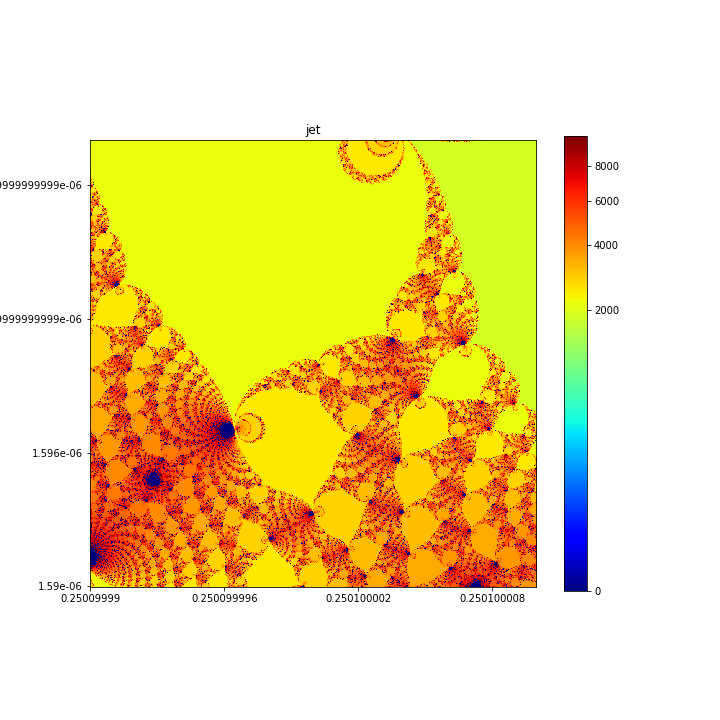
\includegraphics[clip,scale=0.3]{../src/figure/fig002.png}
    \end{minipage}
  \end{tabular}
  \begin{tabular}{cc}
    \begin{minipage}{0.5\hsize}
      \centering
      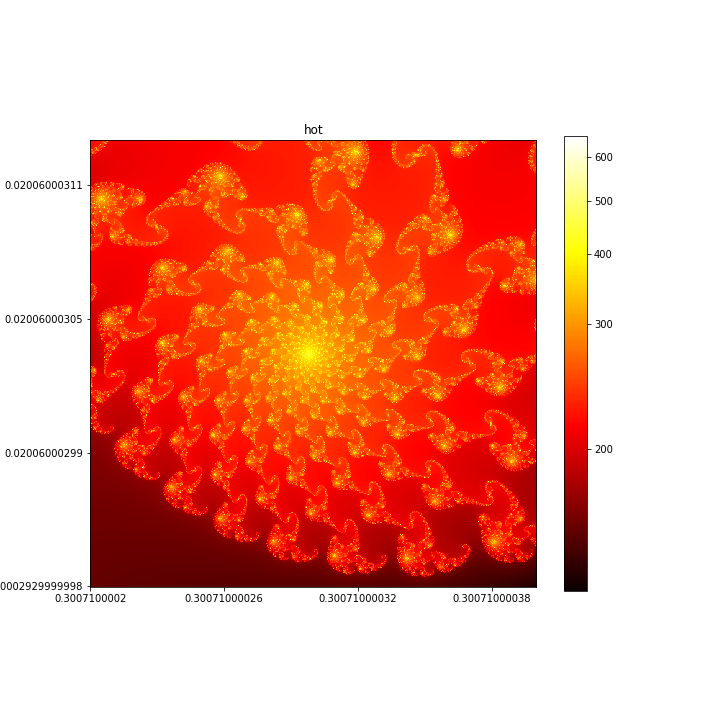
\includegraphics[clip,scale=0.3]{../src/figure/fig003.png}
    \end{minipage}
    \begin{minipage}{0.5\hsize}
      \centering
      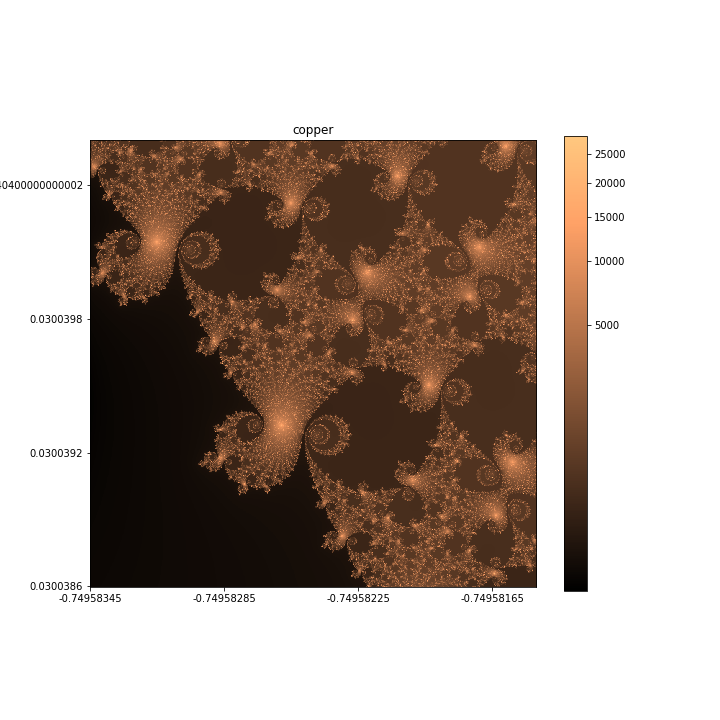
\includegraphics[clip,scale=0.3]{../src/figure/fig004.png}
    \end{minipage}
  \end{tabular}
  \begin{tabular}{cc}
    \begin{minipage}{0.5\hsize}
      \centering
      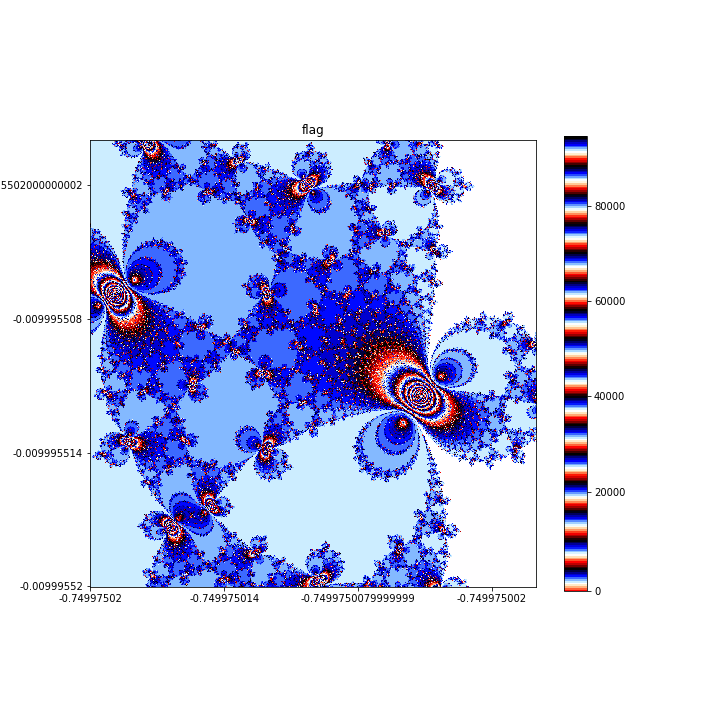
\includegraphics[clip,scale=0.3]{../src/figure/fig005.png}
    \end{minipage}
    \begin{minipage}{0.5\hsize}
      \centering
      %\includegraphics[clip,scale=0.4]{figure2.png}
    \end{minipage}
  \end{tabular}
\end{figure}%

%
\section*{謝辞}
\addcontentsline{toc}{chapter}{謝辞}
%
\begin{thebibliography}{99}
  \bibitem{1} B.Mandelbrot 著、広中平祐 監訳 『フラクタル幾何学』第1版(日経サイエンス社 1986)
  \bibitem{2} 宇敷重広『フラクタルの世界』第1版(日本評論社 1987)
  \bibitem{3} 渕上季代絵『フラクタルCGコレクション』第2版(サイエンス社 1987)
  \bibitem{4} 佃勉『フラクタルの世界』第1版(山海堂 1987)
  \bibitem{5} 佐藤幸悦『フラクタル・グラフィックス』(ラッセル社 1989)
  \bibitem{6} Amit Saha 著、黒川利明 訳 『Pythonからはじめる数学入門』初版(オライリー・ジャパン 2016)
  \bibitem{7} 奥村晴彦,黒木裕介『\LaTeXe 美文書作成入門』第7版(技術評論社,2017)
\end{thebibliography}
%
% END DOCUMENT
\end{document}
%
